\documentclass[11pt]{article}
\usepackage[margin=0.9in]{geometry}
\usepackage{amsmath,amssymb}
\usepackage{graphicx}
\usepackage{hyperref}
\usepackage{enumitem}
\usepackage{booktabs}
\usepackage{caption}
\usepackage{xcolor}

\graphicspath{{figures/}}
\captionsetup{font=small,labelfont=bf,skip=6pt}

\title{Summary:\\COSMA: Communication-aware Optimization of\\Fermionic Simulation Kernels for Modular Quantum Architectures}
\author{Enrico Russo, Francesco G. Blanco, Elio Vinciguerra,\\Davide Patti, Giuseppe Ascia, Maurizio Palesi\\
\textit{arXiv:2607.09381} (IEEE QCE 2026)}
\date{}

\begin{document}
\maketitle

%% ============================================================
\section{Main new idea}
%% ============================================================

On modular / multi-core QPUs, fermionic simulation (Trotterized chemistry) is bottlenecked by
\textbf{inter-core qubit state transfers}, not local gates.
Prior compilers typically fix a fermion-to-qubit (F2Q) mapping (JW, BK, \ldots), synthesize Pauli
gadgets, then allocate qubits --- treating those stages separately.

\textbf{COSMA}'s new idea is joint, communication-aware co-design of three coupled stages:
\begin{enumerate}[leftmargin=*,itemsep=2pt]
  \item a \textbf{genetic search over product-preserving ternary-tree (PPTT) F2Q mappings}
        (tree shape + mode order), with fitness $=$ downstream transfer cost;
  \item \textbf{Pauli scheduling} that smooths support changes (Gray-inspired best);
  \item a \textbf{parity-tree synthesis + multi-core allocator} that builds CNOT trees
        core-by-core and merges them with a lookahead misplacement score.
\end{enumerate}
On 14 molecular STO-3G benchmarks (14--90 modes, cores of capacity 8), COSMA reports up to
$\sim\!2.5\times$ lower communication cost vs.\ fixed-mapping + Hungarian allocation baselines
(median $\sim\!1.7\times$ / $\sim\!60\%$ reduction under Gray scheduling).

%% ============================================================
\section{Toy model with concrete numbers}
%% ============================================================

\subsection*{Setup}
Two cores $C_0$--$C_1$ linked by distance $d=1$, capacity $\kappa=4$ each.
$N=6$ qubits. One Trotter step has $T=4$ Pauli gadgets with supports
\[
\begin{aligned}
S_1&=\{1,2,3\},&
S_2&=\{1,2,4\},&
S_3&=\{4,5,6\},&
S_4&=\{3,5,6\}.
\end{aligned}
\]
Communication cost (paper Eq.~(14)) counts total core-distance moved by every qubit
between consecutive slices.

\subsection*{Naive pipeline (JW + magnitude + fixed CNOT chain + Hungarian)}
JW mapping spreads modes so supports straddle cores often.
Magnitude ordering ignores support smoothness:
support-delta surrogate (Eq.~(19))
\[
\Delta_{\mathrm{sched}}=\sum_{t=2}^{T}|S_{t-1}\triangle S_t|
= |\{3\}\triangle\{4\}| + |\{1,2\}\triangle\{5,6\}| + |\{4\}\triangle\{3\}|
= 2+4+2=8.
\]
Each gadget needs a parity tree merged across cores $\Rightarrow$ roughly 2 transfers per
gadget $\times$ forward+reverse $\approx 16$ unit-distance transfers.
\textbf{Naive cost $\approx 16$.}

\subsection*{COSMA-style choices}
\begin{itemize}[leftmargin=*,itemsep=2pt]
  \item Mapping places modes so $S_1,S_2$ live mostly on $C_0$ and $S_3,S_4$ on $C_1$.
  \item Gray-inspired order: $(S_1,S_2,S_4,S_3)$ so consecutive supports change by
        only 1--2 qubits: $\Delta_{\mathrm{sched}}=2+2+2=6$ (25\% smoother).
  \item Allocator builds a local parity chain inside each core, then merges at one
        meeting core; lookahead keeps well-placed qubits still.
\end{itemize}
Suppose transfers drop to 6 unit moves.
\textbf{COSMA cost $\approx 6$} --- about $\mathbf{2.7\times}$ cheaper, in the same ballpark as
the paper's peak $\sim\!2.5\times$ / median $\sim\!1.7\times$.

\begin{center}
\begin{tabular}{@{}lrrr@{}}
\toprule
Pipeline & $\Delta_{\mathrm{sched}}$ & Transfers & Cost ratio \\
\midrule
JW+MAG+HQA (naive) & 8 & 16 & 1.00 \\
COSMA map+GRAY+co-alloc & 6 & 6 & $\mathbf{0.38}$ ($\sim\!2.6\times$) \\
\bottomrule
\end{tabular}
\end{center}

%% ============================================================
\section{Paper math walkthrough}
%% ============================================================

\subsection*{Simulation kernel}
Electronic Hamiltonian $\to$ Majorana form $\to$ Pauli sum
\begin{equation}
H=\sum_j \alpha_j P_j,\qquad
e^{-iHt}\approx\Bigg(\prod_j e^{-i\alpha_j P_j t/r}\Bigg)^r.
\end{equation}
Each factor $e^{-i\theta P}$ is a \textbf{Pauli gadget}: basis change $\to$ CNOT parity tree
$\to R_Z(2\theta)$ on the root $\to$ reverse tree.

\subsection*{Objective (what COSMA minimizes)}
With layout $\ell_l(q)=$ core of qubit $q$ in slice $l$,
\begin{equation}
\mathrm{cost}(\mathcal{M},\pi,\{\mathcal{T}_t\},\{\ell_l\})
=\sum_{l=1}^{L-1}\sum_{q=1}^{N} d\!\big(\ell_l(q),\ell_{l+1}(q)\big),
\label{eq:cost}
\end{equation}
and
\begin{equation}
\min_{\mathcal{M},\pi,\{\mathcal{T}_t\},\{\ell_l\}}
\mathrm{cost}(\mathcal{M},\pi,\{\mathcal{T}_t\},\{\ell_l\}).
\end{equation}
Symbols: $\mathcal{M}$~PPTT F2Q mapping; $\pi$~Pauli order; $\mathcal{T}_t$~parity tree for term~$t$;
$d$~shortest-path core distance.

\subsection*{Why mapping matters}
PPTT search space size is $A_N^{(3)}\cdot N!$ with ternary Fuss--Catalan
$A_N^{(3)}=\frac{1}{2N+1}\binom{3N}{N}$. Different trees change Pauli supports $S_t$,
hence which gadgets cross cores.

\subsection*{Gray scheduling surrogate}
With support mask $M_t$,
\begin{equation}
g(P)=M(P)\oplus\big(M(P)\gg 1\big),\qquad
\Delta_{\mathrm{sched}}=\sum_{t=2}^{T} d_H(M_{t-1},M_t).
\end{equation}
Sorting by $g(P)$ clusters similar supports --- fewer qubits to reshuffle.

\subsection*{Allocator lookahead}
Misplacement of qubit $q$ at term $t$ (window $W$, discount $\gamma$):
\begin{equation}
\bar d_t(q)=\sum_{\tau\in W_t(q)}\gamma^{\tau-t}\,\delta_\tau(q),
\end{equation}
where $\delta_\tau(q)$ is average core-distance from $q$ to co-support partners.
Meeting core for term~$t$:
\begin{equation}
c_t^\star=\arg\min_{c\in A(S_t)}\sum_{q\in S_t}\frac{d\big(c,\ell_t(q)\big)}{1+\bar d_t(q)}.
\end{equation}
Forward merge + backward co-location use these scores to decide which qubit moves when
parity subtrees on different cores must be joined --- mapping toy transfers onto Eq.~\eqref{eq:cost}.

%% ============================================================
\section{Figures from the paper}
%% ============================================================

\begin{figure}[ht]
\centering
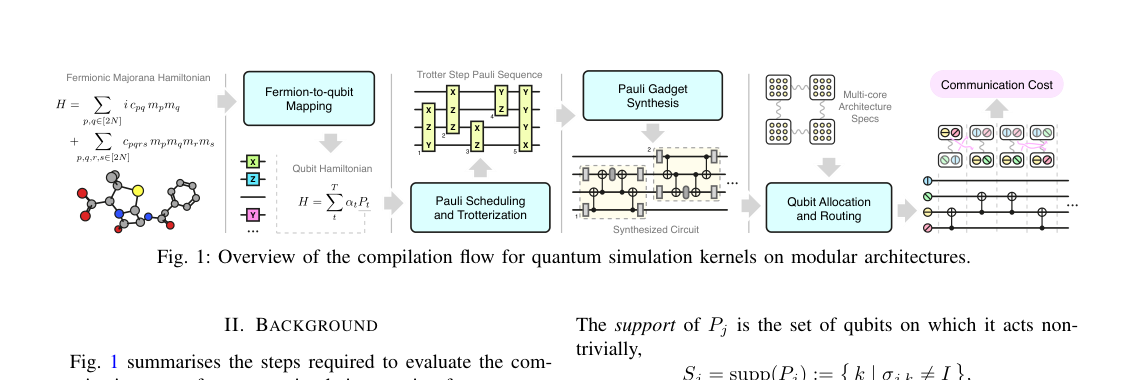
\includegraphics[width=\textwidth]{fig1_overview.png}
\caption{\textbf{FIG.~1 (paper) --- compilation flow.}
Molecule $\to$ F2Q mapping $\to$ Pauli Hamiltonian $\to$ scheduled Trotter sequence $\to$
Pauli-gadget synthesis $\to$ qubit allocation/routing on a multi-core grid $\to$
\textbf{communication cost} (inter-core state transfers).}
\end{figure}

\noindent\textit{How to read Fig.~1.}
Every arrow is a compiler stage COSMA co-optimizes. The rightmost ``Communication Cost''
panel is the fitness signal fed back into the genetic F2Q search.

\begin{figure}[ht]
\centering
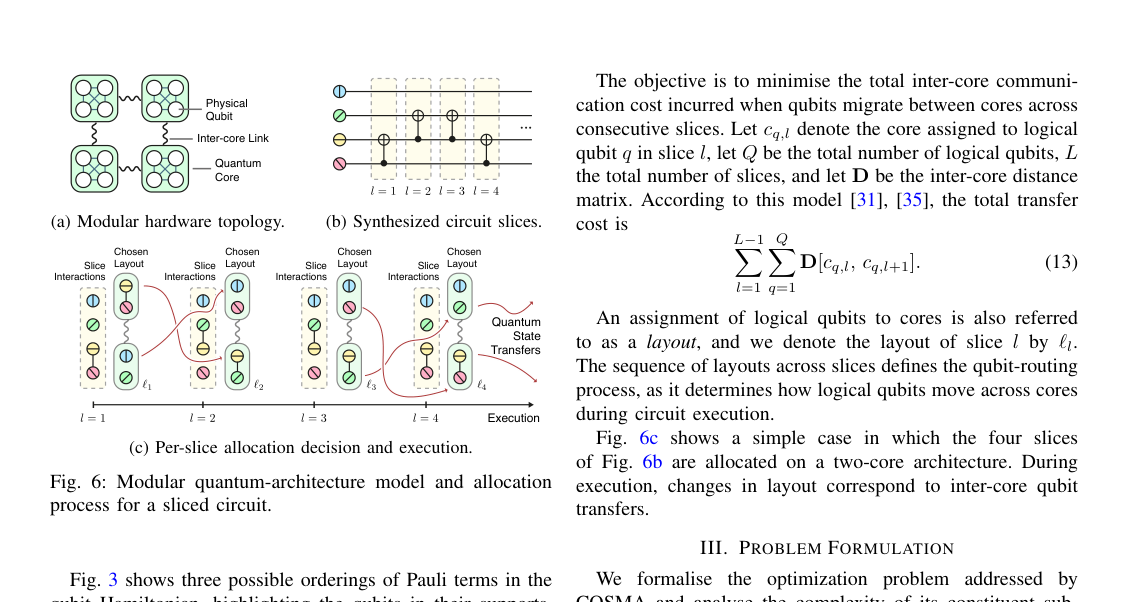
\includegraphics[width=\textwidth]{fig6_modular.png}
\caption{\textbf{FIG.~6 (paper) --- modular model + sliced allocation.}
\textbf{(a)}~Cores with local qubits and inter-core links.
\textbf{(b)}~Circuit sliced into parallel CNOT groups.
\textbf{(c)}~Per-slice layouts; red arcs $=$ quantum state transfers when a qubit's core changes.}
\end{figure}

\noindent\textit{How to read Fig.~6.}
Cost Eq.~\eqref{eq:cost} literally counts those red arcs (weighted by link distance).
COSMA's job is to choose mapping, order, and trees so fewer arcs appear.

\begin{figure}[ht]
\centering
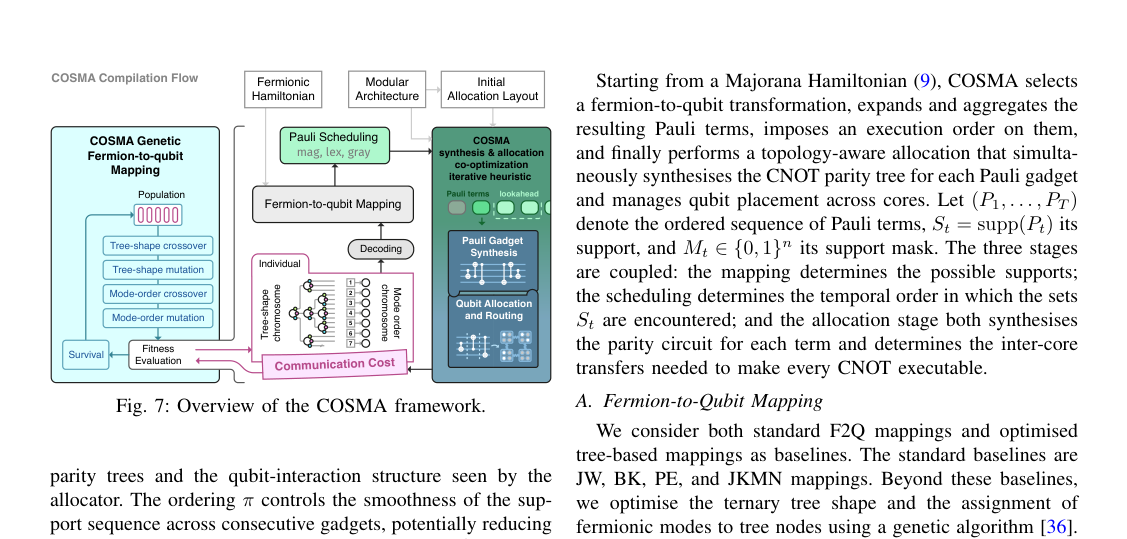
\includegraphics[width=\textwidth]{fig7_framework.png}
\caption{\textbf{FIG.~7 (paper) --- COSMA framework.}
Genetic individuals $=$ (tree-shape chromosome, mode-order chromosome).
Fitness $=$ full schedule+allocate cost. Downstream: mag/lex/gray scheduling and
iterative synthesis/allocation with lookahead.}
\end{figure}

\noindent\textit{How to read Fig.~7.}
The loop ``Population $\to$ Fitness (communication cost) $\to$ Survival'' is the novelty:
mapping is scored by modular communication, not Pauli weight alone.

\begin{figure}[ht]
\centering
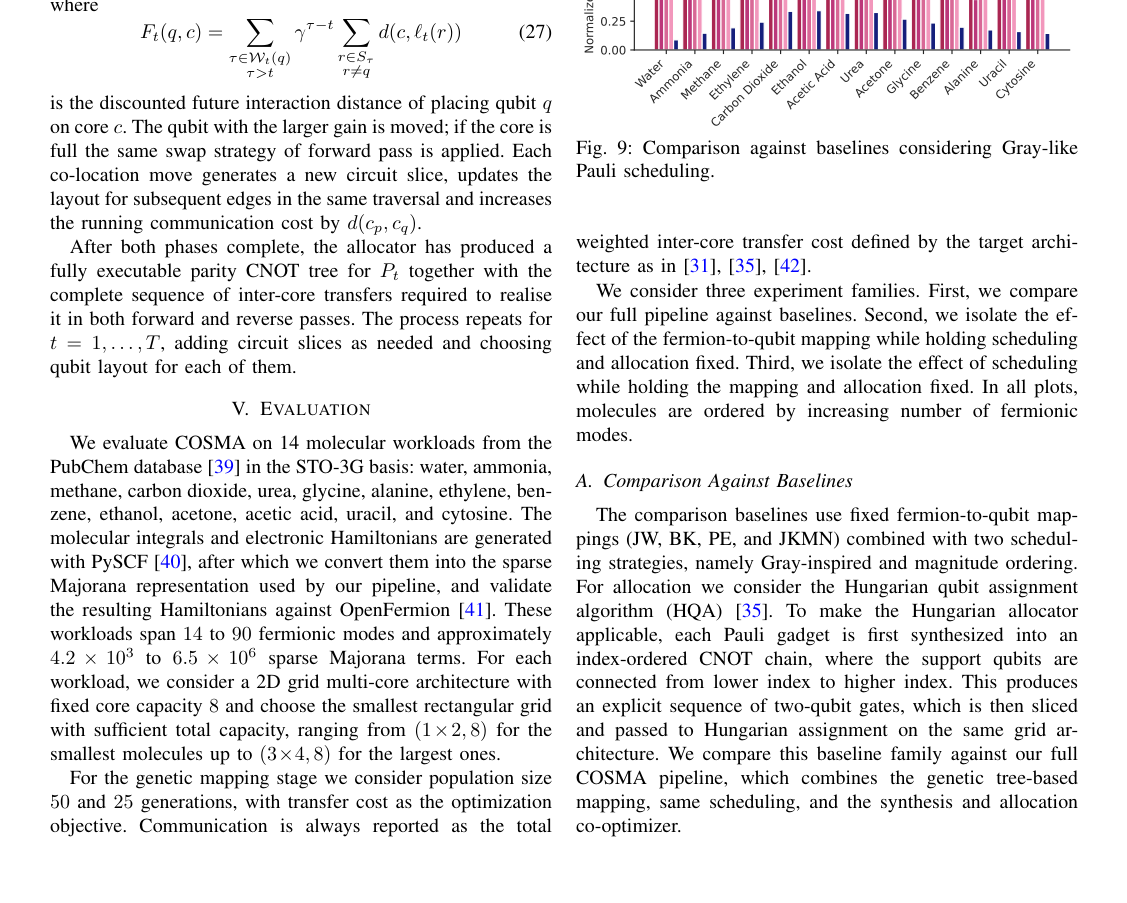
\includegraphics[width=\textwidth]{fig8_9_both.png}
\caption{\textbf{FIGS.~8--9 (paper) --- full pipeline vs.\ baselines.}
Normalized inter-core transfer cost across 14 molecules (Water$\to$Cytosine).
Pink/red bars: fixed JW/BK/PE/JKMN + HQA. Dark blue: full COSMA.
Fig.~8 uses magnitude scheduling; Fig.~9 uses Gray-inspired (median $\mathbf{59.7\%}$ reduction).}
\end{figure}

\noindent\textit{How to read Figs.~8--9.}
Shorter blue bars $=$ fewer state transfers. Advantage holds from 14-mode water to
$\sim\!90$-mode cytosine. Abstract's ``up to $2.5\times$ / median $1.7\times$'' is this gap
rephrased as a speedup factor.

\begin{figure}[ht]
\centering
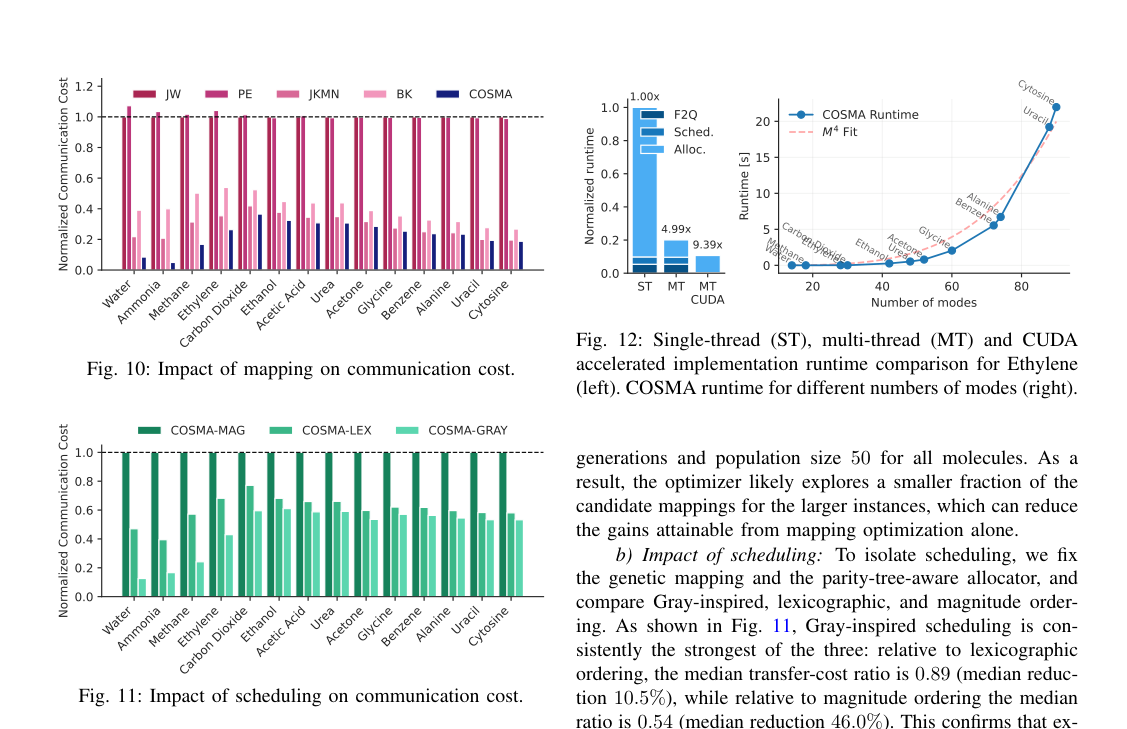
\includegraphics[width=\textwidth]{fig10_11_12.png}
\caption{\textbf{FIGS.~10--12 (paper) --- ablations + runtime.}
\textbf{Fig.~10:} mapping-only ablation (same Gray scheduler + COSMA allocator): genetic
PPTT mapping median $\mathbf{11.4\%}$ better than best fixed mapping.
\textbf{Fig.~11:} scheduling-only ablation: GRAY beats LEX by $\sim\!10.5\%$ and MAG by
$\sim\!46\%$ (median).
\textbf{Fig.~12:} runtime --- CUDA $\sim\!9.4\times$ vs.\ single-thread; scales $\sim M^4$ with modes.}
\end{figure}

\noindent\textit{How to read Figs.~10--12.}
Most of the big win in Figs.~8--9 is joint co-optimization (allocator+mapping together),
not mapping alone (only $+11\%$). Scheduling choice is large when the allocator is fixed:
smooth supports (GRAY) matter. Fig.~12 says the GA is practical with GPU for the inner loop.

%% ============================================================
\section{Takeaway}
%% ============================================================

COSMA's novelty is treating \textbf{F2Q mapping, Pauli order, and parity-tree/allocation as one
communication objective} for modular chemistry kernels.
The concrete win is fewer inter-core teleports/transfers (up to $\sim\!2.5\times$), driven especially
by Gray-smoothed schedules plus a lookahead parity-forest allocator --- with a genetic PPTT
mapper using that cost as fitness.

\end{document}
